\documentclass[11pt]{article}

\author{Math 123}
\date{Due March 16, 2023 by midnight} 
\title{Homework 7}

\usepackage{graphicx,xypic}
\usepackage{amsthm}
\usepackage{amsmath,amssymb}
\usepackage{amsfonts}
\usepackage{xcolor}
\usepackage[margin=1in]{geometry}
\usepackage[shortlabels]{enumitem}
\newtheorem{problem}{Problem}
\renewcommand*{\proofname}{{\color{blue}Solution}}


\usepackage{fancyhdr}
\pagestyle{fancy}
\rhead{Math 123, Homework 7}

\setlength{\parindent}{0pt}
\setlength{\parskip}{1.25ex}

% tikz
\usepackage{tikz}
\usetikzlibrary{intersections, angles, quotes, positioning}
\usetikzlibrary{arrows.meta}
\usepackage{pgfplots}
\pgfplotsset{compat=1.13}


\tikzset{
	force/.style={thick, {Circle[length=2pt]}-stealth, shorten <=-1pt}
}

% quiver style
\usepackage{tikz-cd}
% `calc` is necessary to draw curved arrows.
\usetikzlibrary{calc}
% `pathmorphing` is necessary to draw squiggly arrows.
\usetikzlibrary{decorations.pathmorphing}

% A TikZ style for curved arrows of a fixed height, due to AndréC.
\tikzset{curve/.style={settings={#1},to path={(\tikztostart)
					.. controls ($(\tikztostart)!\pv{pos}!(\tikztotarget)!\pv{height}!270:(\tikztotarget)$)
					and ($(\tikztostart)!1-\pv{pos}!(\tikztotarget)!\pv{height}!270:(\tikztotarget)$)
					.. (\tikztotarget)\tikztonodes}},
	settings/.code={\tikzset{quiver/.cd,#1}
			\def\pv##1{\pgfkeysvalueof{/tikz/quiver/##1}}},
	quiver/.cd,pos/.initial=0.35,height/.initial=0}

% TikZ arrowhead/tail styles.
\tikzset{tail reversed/.code={\pgfsetarrowsstart{tikzcd to}}}
\tikzset{2tail/.code={\pgfsetarrowsstart{Implies[reversed]}}}
\tikzset{2tail reversed/.code={\pgfsetarrowsstart{Implies}}}
% TikZ arrow styles.
\tikzset{no body/.style={/tikz/dash pattern=on 0 off 1mm}}

\begin{document}

\maketitle

% You are required to put your name here:
{\bf\Large Name: George Chemmala} 


\vspace{.3in}
Topics covered: Graph coloring, chromatic polynomial, Turan graphs

Instructions: 
\begin{itemize}
\item This assignment must be submitted on Gradescope by the due date. 
\item If you collaborate with other students (which is encouraged!), please mention this somewhere on the assignment. 
\item If you are stuck, please ask for help (from me, a TA, a classmate). Use Campuswire!  
\item You may freely use any fact proved in class. In general, you should provide proof for facts used that were not proved in class. 
\item Please restrict your solution to each problem to a single page. Usually solutions can be even shorter than that. If your solution is very long, you should think more about how to express it concisely.
\end{itemize}


\pagebreak 


\begin{problem}
Give an example or explain why no example exists: A graph $G$ that is neither complete nor an odd cycle, but for which the greedy coloring uses $\Delta(G)+1$ colors. 
\end{problem}

\begin{proof}
Counterexample:
    % https://q.uiver.app/?q=WzAsNCxbMCwwLCIxIl0sWzEsMCwiNCJdLFsyLDAsIjMiXSxbMywwLCIyIl0sWzAsMSwiIiwwLHsic3R5bGUiOnsiaGVhZCI6eyJuYW1lIjoibm9uZSJ9fX1dLFsxLDIsIiIsMCx7InN0eWxlIjp7ImhlYWQiOnsibmFtZSI6Im5vbmUifX19XSxbMiwzLCIiLDAseyJzdHlsZSI6eyJoZWFkIjp7Im5hbWUiOiJub25lIn19fV1d
\[\begin{tikzcd}
	1 & 4 & 3 & 2
	\arrow[no head, from=1-1, to=1-2]
	\arrow[no head, from=1-2, to=1-3]
	\arrow[no head, from=1-3, to=1-4]
\end{tikzcd}\]

Let \(a,b,c\) be the colorings in alphabetic order \(a \leq b \leq c\)
then
\begin{enumerate}
    \item[1] is colored \(a\) since \(a\) is the minimum coloring and it has no colored neighbors
\[\begin{tikzcd}
	a & 4 & 3 & 2
	\arrow[no head, from=1-2, to=1-3]
	\arrow[no head, from=1-3, to=1-4]
	\arrow[no head, from=1-1, to=1-2]
\end{tikzcd}\]
    \item[2] is colored \(a\) since \(a\) is the minimum coloring and it has no colored neighbors
\[\begin{tikzcd}
	a & 4 & 3 & a
	\arrow[no head, from=1-2, to=1-3]
	\arrow[no head, from=1-3, to=1-4]
	\arrow[no head, from=1-1, to=1-2]
\end{tikzcd}\]
    \item[3] is colored \(b\) since \(a\) is used by its neighbor \(2\)
\[\begin{tikzcd}
	a & 4 & b & a
	\arrow[no head, from=1-2, to=1-3]
	\arrow[no head, from=1-3, to=1-4]
	\arrow[no head, from=1-1, to=1-2]
\end{tikzcd}\]
    \item[4] is colored \(c\) since \(a\) is used by its neighbor \(1\) and \(b\) is used by its neighbor \(3\)
\[\begin{tikzcd}
	a & c & b & a
	\arrow[no head, from=1-2, to=1-3]
	\arrow[no head, from=1-3, to=1-4]
	\arrow[no head, from=1-1, to=1-2]
\end{tikzcd}\]
\end{enumerate} 

\end{proof}

\pagebreak

\begin{problem}
Give a very short proof that the following two graphs have the same chromatic number.\footnote{Note: solutions that construct optimal colorings of these graphs will not receive credit.}
\begin{center}
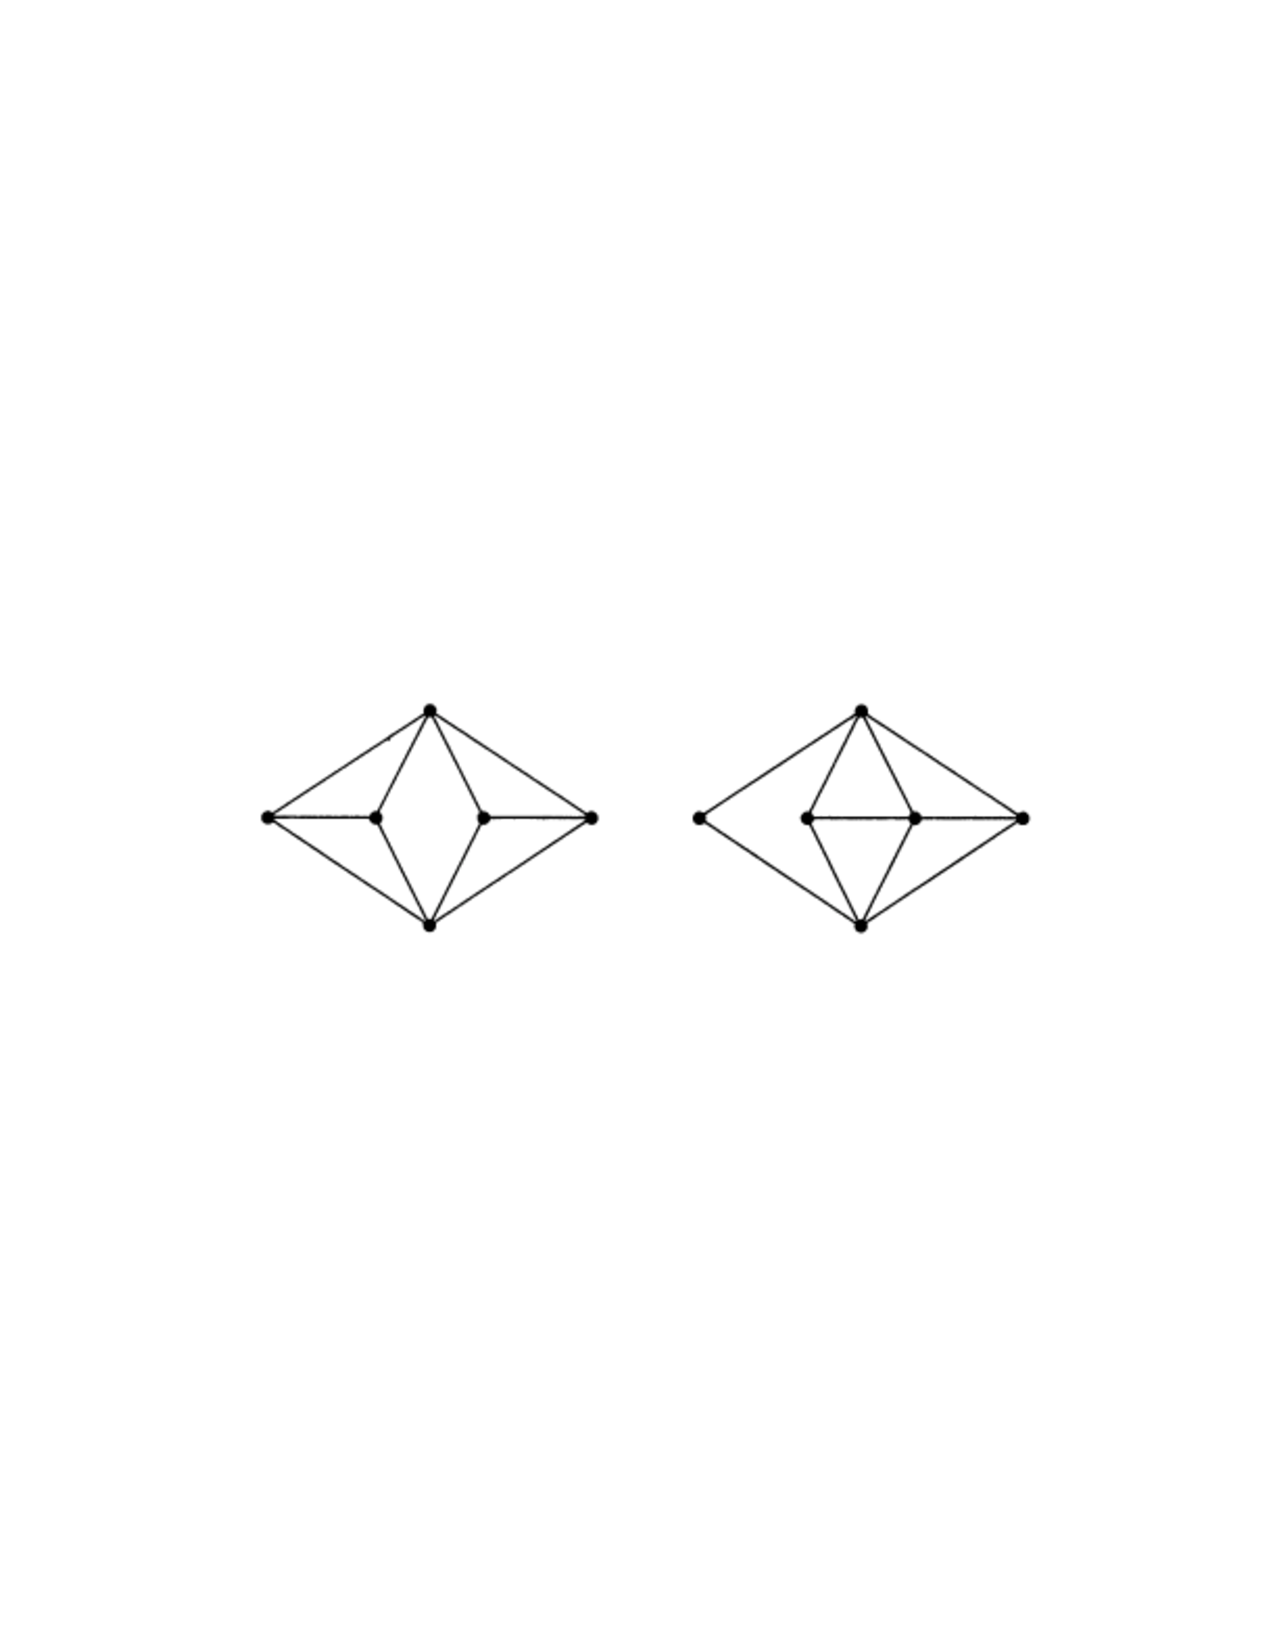
\includegraphics[scale=.5]{hw7-graph.pdf}
\end{center}
\end{problem}

\begin{proof}
Let the left graph be called \(G_1\) and the right graph be called \(G_2\). We know that \(\chi (G, t) = \chi (G \setminus e , t) - \chi (G \cdot e, t)\). Therefore, we can show the two graphs are have the same chromatic polynomial if they both have edges \(e_1, e_2\) s.t. 
\[
	\chi (G_1, t) = 
	\chi (G_1 \setminus e_1 , t) - \chi (G_1 \cdot e_1, t) = 
	\chi (G_2 \setminus e_2 , t) - \chi (G_2 \cdot e_2, t) = 
	\chi (G_2, t)
\]
where \(G_1 \setminus e_1 = G_2 \setminus e_2\) and \(G_1 \cdot e_1 = G_2 \cdot e_2\) by selecting \(e_1\) and \(e_2\) as shown below:

% https://q.uiver.app/?q=WzAsMTIsWzIsMCwiXFxidWxsZXQiXSxbMSwxLCJcXGJ1bGxldCJdLFswLDEsIlxcYnVsbGV0Il0sWzMsMSwiXFxidWxsZXQiXSxbNCwxLCJcXGJ1bGxldCJdLFsyLDIsIlxcYnVsbGV0Il0sWzgsMCwiXFxidWxsZXQiXSxbNiwxLCJcXGJ1bGxldCJdLFs3LDEsIlxcYnVsbGV0Il0sWzksMSwiXFxidWxsZXQiXSxbMTAsMSwiXFxidWxsZXQiXSxbOCwyLCJcXGJ1bGxldCJdLFswLDEsIiIsMCx7InN0eWxlIjp7ImhlYWQiOnsibmFtZSI6Im5vbmUifX19XSxbMCwyLCIiLDIseyJzdHlsZSI6eyJoZWFkIjp7Im5hbWUiOiJub25lIn19fV0sWzAsMywiIiwyLHsic3R5bGUiOnsiaGVhZCI6eyJuYW1lIjoibm9uZSJ9fX1dLFswLDQsIiIsMix7InN0eWxlIjp7ImhlYWQiOnsibmFtZSI6Im5vbmUifX19XSxbNCw1LCIiLDIseyJzdHlsZSI6eyJoZWFkIjp7Im5hbWUiOiJub25lIn19fV0sWzIsNSwiIiwxLHsic3R5bGUiOnsiaGVhZCI6eyJuYW1lIjoibm9uZSJ9fX1dLFs1LDEsIiIsMSx7InN0eWxlIjp7ImhlYWQiOnsibmFtZSI6Im5vbmUifX19XSxbNSwzLCIiLDEseyJzdHlsZSI6eyJoZWFkIjp7Im5hbWUiOiJub25lIn19fV0sWzYsNywiIiwxLHsic3R5bGUiOnsiaGVhZCI6eyJuYW1lIjoibm9uZSJ9fX1dLFs2LDgsIiIsMSx7InN0eWxlIjp7ImhlYWQiOnsibmFtZSI6Im5vbmUifX19XSxbNiw5LCIiLDEseyJzdHlsZSI6eyJoZWFkIjp7Im5hbWUiOiJub25lIn19fV0sWzYsMTAsIiIsMSx7InN0eWxlIjp7ImhlYWQiOnsibmFtZSI6Im5vbmUifX19XSxbOCw5LCJlXzIiLDEseyJzdHlsZSI6eyJoZWFkIjp7Im5hbWUiOiJub25lIn19fV0sWzksMTAsIiIsMSx7InN0eWxlIjp7ImhlYWQiOnsibmFtZSI6Im5vbmUifX19XSxbMTAsMTEsIiIsMSx7InN0eWxlIjp7ImhlYWQiOnsibmFtZSI6Im5vbmUifX19XSxbMTEsOSwiIiwxLHsic3R5bGUiOnsiaGVhZCI6eyJuYW1lIjoibm9uZSJ9fX1dLFsxMSw4LCIiLDEseyJzdHlsZSI6eyJoZWFkIjp7Im5hbWUiOiJub25lIn19fV0sWzExLDcsIiIsMSx7InN0eWxlIjp7ImhlYWQiOnsibmFtZSI6Im5vbmUifX19XSxbMiwxLCJlXzEiLDEseyJzdHlsZSI6eyJoZWFkIjp7Im5hbWUiOiJub25lIn19fV0sWzMsNCwiIiwwLHsic3R5bGUiOnsiaGVhZCI6eyJuYW1lIjoibm9uZSJ9fX1dXQ==
\[\begin{tikzcd}
	&& \bullet &&&&&& \bullet \\
	\bullet & \bullet && \bullet & \bullet && \bullet & \bullet && \bullet & \bullet \\
	&& \bullet &&&&&& \bullet
	\arrow[no head, from=1-3, to=2-2]
	\arrow[no head, from=1-3, to=2-1]
	\arrow[no head, from=1-3, to=2-4]
	\arrow[no head, from=1-3, to=2-5]
	\arrow[no head, from=2-5, to=3-3]
	\arrow[no head, from=2-1, to=3-3]
	\arrow[no head, from=3-3, to=2-2]
	\arrow[no head, from=3-3, to=2-4]
	\arrow[no head, from=1-9, to=2-7]
	\arrow[no head, from=1-9, to=2-8]
	\arrow[no head, from=1-9, to=2-10]
	\arrow[no head, from=1-9, to=2-11]
	\arrow["{e_2}"{description}, no head, from=2-8, to=2-10]
	\arrow[no head, from=2-10, to=2-11]
	\arrow[no head, from=2-11, to=3-9]
	\arrow[no head, from=3-9, to=2-10]
	\arrow[no head, from=3-9, to=2-8]
	\arrow[no head, from=3-9, to=2-7]
	\arrow["{e_1}"{description}, no head, from=2-1, to=2-2]
	\arrow[no head, from=2-4, to=2-5]
\end{tikzcd}\]

Here is some work of showing the equivalence of the statements.

\(G_1 \setminus e_1 = G_2 \setminus e_2\):
 % https://q.uiver.app/?q=WzAsMTIsWzIsMCwiXFxidWxsZXQiXSxbMSwxLCJcXGJ1bGxldCJdLFswLDEsIlxcYnVsbGV0Il0sWzMsMSwiXFxidWxsZXQiXSxbNCwxLCJcXGJ1bGxldCJdLFsyLDIsIlxcYnVsbGV0Il0sWzgsMCwiXFxidWxsZXQiXSxbNiwxLCJcXGJ1bGxldCJdLFs3LDEsIlxcYnVsbGV0Il0sWzksMSwiXFxidWxsZXQiXSxbMTAsMSwiXFxidWxsZXQiXSxbOCwyLCJcXGJ1bGxldCJdLFswLDEsIiIsMCx7InN0eWxlIjp7ImhlYWQiOnsibmFtZSI6Im5vbmUifX19XSxbMCwyLCIiLDIseyJzdHlsZSI6eyJoZWFkIjp7Im5hbWUiOiJub25lIn19fV0sWzAsMywiIiwyLHsic3R5bGUiOnsiaGVhZCI6eyJuYW1lIjoibm9uZSJ9fX1dLFswLDQsIiIsMix7InN0eWxlIjp7ImhlYWQiOnsibmFtZSI6Im5vbmUifX19XSxbNCw1LCIiLDIseyJzdHlsZSI6eyJoZWFkIjp7Im5hbWUiOiJub25lIn19fV0sWzIsNSwiIiwxLHsic3R5bGUiOnsiaGVhZCI6eyJuYW1lIjoibm9uZSJ9fX1dLFs1LDEsIiIsMSx7InN0eWxlIjp7ImhlYWQiOnsibmFtZSI6Im5vbmUifX19XSxbNSwzLCIiLDEseyJzdHlsZSI6eyJoZWFkIjp7Im5hbWUiOiJub25lIn19fV0sWzYsNywiIiwxLHsic3R5bGUiOnsiaGVhZCI6eyJuYW1lIjoibm9uZSJ9fX1dLFs2LDgsIiIsMSx7InN0eWxlIjp7ImhlYWQiOnsibmFtZSI6Im5vbmUifX19XSxbNiw5LCIiLDEseyJzdHlsZSI6eyJoZWFkIjp7Im5hbWUiOiJub25lIn19fV0sWzYsMTAsIiIsMSx7InN0eWxlIjp7ImhlYWQiOnsibmFtZSI6Im5vbmUifX19XSxbOSwxMCwiIiwxLHsic3R5bGUiOnsiaGVhZCI6eyJuYW1lIjoibm9uZSJ9fX1dLFsxMCwxMSwiIiwxLHsic3R5bGUiOnsiaGVhZCI6eyJuYW1lIjoibm9uZSJ9fX1dLFsxMSw5LCIiLDEseyJzdHlsZSI6eyJoZWFkIjp7Im5hbWUiOiJub25lIn19fV0sWzExLDgsIiIsMSx7InN0eWxlIjp7ImhlYWQiOnsibmFtZSI6Im5vbmUifX19XSxbMTEsNywiIiwxLHsic3R5bGUiOnsiaGVhZCI6eyJuYW1lIjoibm9uZSJ9fX1dLFszLDQsIiIsMCx7InN0eWxlIjp7ImhlYWQiOnsibmFtZSI6Im5vbmUifX19XV0=
\[\begin{tikzcd}
	&& \bullet &&&&&& \bullet \\
	\bullet & \bullet && \bullet & \bullet && \bullet & \bullet && \bullet & \bullet \\
	&& \bullet &&&&&& \bullet
	\arrow[no head, from=1-3, to=2-2]
	\arrow[no head, from=1-3, to=2-1]
	\arrow[no head, from=1-3, to=2-4]
	\arrow[no head, from=1-3, to=2-5]
	\arrow[no head, from=2-5, to=3-3]
	\arrow[no head, from=2-1, to=3-3]
	\arrow[no head, from=3-3, to=2-2]
	\arrow[no head, from=3-3, to=2-4]
	\arrow[no head, from=1-9, to=2-7]
	\arrow[no head, from=1-9, to=2-8]
	\arrow[no head, from=1-9, to=2-10]
	\arrow[no head, from=1-9, to=2-11]
	\arrow[no head, from=2-10, to=2-11]
	\arrow[no head, from=2-11, to=3-9]
	\arrow[no head, from=3-9, to=2-10]
	\arrow[no head, from=3-9, to=2-8]
	\arrow[no head, from=3-9, to=2-7]
	\arrow[no head, from=2-4, to=2-5]
\end{tikzcd}\]

\(G_1 \cdot e_1 = G_2 \cdot e_2\):
% https://q.uiver.app/?q=WzAsMTAsWzIsMCwiXFxidWxsZXQiXSxbMCwxLCJcXGJ1bGxldCJdLFszLDEsIlxcYnVsbGV0Il0sWzQsMSwiXFxidWxsZXQiXSxbMiwyLCJcXGJ1bGxldCJdLFs4LDAsIlxcYnVsbGV0Il0sWzYsMSwiXFxidWxsZXQiXSxbOSwxLCJcXGJ1bGxldCJdLFsxMCwxLCJcXGJ1bGxldCJdLFs4LDIsIlxcYnVsbGV0Il0sWzAsMSwiIiwyLHsic3R5bGUiOnsiaGVhZCI6eyJuYW1lIjoibm9uZSJ9fX1dLFswLDIsIiIsMix7InN0eWxlIjp7ImhlYWQiOnsibmFtZSI6Im5vbmUifX19XSxbMCwzLCIiLDIseyJzdHlsZSI6eyJoZWFkIjp7Im5hbWUiOiJub25lIn19fV0sWzMsNCwiIiwyLHsic3R5bGUiOnsiaGVhZCI6eyJuYW1lIjoibm9uZSJ9fX1dLFsxLDQsIiIsMSx7InN0eWxlIjp7ImhlYWQiOnsibmFtZSI6Im5vbmUifX19XSxbNCwyLCIiLDEseyJzdHlsZSI6eyJoZWFkIjp7Im5hbWUiOiJub25lIn19fV0sWzUsNiwiIiwxLHsic3R5bGUiOnsiaGVhZCI6eyJuYW1lIjoibm9uZSJ9fX1dLFs1LDcsIiIsMSx7InN0eWxlIjp7ImhlYWQiOnsibmFtZSI6Im5vbmUifX19XSxbNSw4LCIiLDEseyJzdHlsZSI6eyJoZWFkIjp7Im5hbWUiOiJub25lIn19fV0sWzcsOCwiIiwxLHsic3R5bGUiOnsiaGVhZCI6eyJuYW1lIjoibm9uZSJ9fX1dLFs4LDksIiIsMSx7InN0eWxlIjp7ImhlYWQiOnsibmFtZSI6Im5vbmUifX19XSxbOSw3LCIiLDEseyJzdHlsZSI6eyJoZWFkIjp7Im5hbWUiOiJub25lIn19fV0sWzksNiwiIiwxLHsic3R5bGUiOnsiaGVhZCI6eyJuYW1lIjoibm9uZSJ9fX1dLFsyLDMsIiIsMCx7InN0eWxlIjp7ImhlYWQiOnsibmFtZSI6Im5vbmUifX19XV0=
\[\begin{tikzcd}
	&& \bullet &&&&&& \bullet \\
	\bullet &&& \bullet & \bullet && \bullet &&& \bullet & \bullet \\
	&& \bullet &&&&&& \bullet
	\arrow[no head, from=1-3, to=2-1]
	\arrow[no head, from=1-3, to=2-4]
	\arrow[no head, from=1-3, to=2-5]
	\arrow[no head, from=2-5, to=3-3]
	\arrow[no head, from=2-1, to=3-3]
	\arrow[no head, from=3-3, to=2-4]
	\arrow[no head, from=1-9, to=2-7]
	\arrow[no head, from=1-9, to=2-10]
	\arrow[no head, from=1-9, to=2-11]
	\arrow[no head, from=2-10, to=2-11]
	\arrow[no head, from=2-11, to=3-9]
	\arrow[no head, from=3-9, to=2-10]
	\arrow[no head, from=3-9, to=2-7]
	\arrow[no head, from=2-4, to=2-5]
\end{tikzcd}\]

\end{proof}

\pagebreak


\begin{problem}
Let $G=M_{n_1,\ldots,n_k}$ be a complete $k$-partite graph with $n=n_1+\cdots+n_r$ vertices. Show that if $n_i-n_j\ge2$ for some $i,j$, then there exists a $k$-partite graph with $n$ vertices and more edges than $G$. 
\end{problem}

\begin{proof}
Continuing the discussion from class, we know that the number of edges of a graph \(M_{n_1 \cdots n_k}\) is the sum of all pairwise products of the size of the coloring groups. And by the symmetry of pairwise products, this implies that the maximum occurs when all groups have the same size. However, since there might be cases where \(r \nmid n\) then each group must size of at most 1 more than any of the other groups, since if it contains 2 more vertices, one of those could be allocated to another group such that all groups are closer to being the same size.

\end{proof}

\pagebreak


\begin{problem}
Given a set of lines in the plane with no three meeting at a point, form a graph $G$ whose vertices are the intersections of the lines, with two vertices adjacent if they appear consecutively on one of the lines. Prove that $\chi(G)\le3$. 
\footnote{Suggestion: start by looking at some explicit examples.} \footnote{Hint: use a greedy coloring with an appropriate vertex ordering.} 
\end{problem}

\begin{proof}
Cases with perpendicular lines can be slanted for the following proof since altering the left/right position of the vertices does not matter.

Since no more than 2 lines intersect to create a point there can be at most 2 neighboring points to the left of any given point. Therefore, we can apply a greedy coloring starting form the left and moving to the right, coloring the 2 neighboring points to the left and then coloring the right point with the 3rd color if the 2 neighboring points are different colors. 
\end{proof}


\pagebreak



\begin{problem}
Let $G$ be a graph with chromatic number $k$. Show that for every $k$-coloring of $G$ and for each color $i$, there is a vertex of color $i$ that is adjacent to vertices of the other $k-1$ colors. \footnote{Hint: think back to the proof that a graph with chromatic number $k$ has at least ${k\choose 2}$ edges.}
\end{problem}

\begin{proof}
Suppose for some \(k\) coloring of \(G\) there does not exist a vertex of color \(i\) s.t. it is adjacent to vertices of the all the other $k-1$ colors. Since no vertex is connected all to the other \(k - 1\) colors then there exists at least one color group that each vertex is not connected to. Therefore, we can take the vertices in the \(i\) colored group and disperse them amongst the other colors, resulting in a coloring of \(G\) with \(k - 1\) colors - a contradiction because \(G\) has chromatic number \(k\).

\emph{Example:}
Here the \(g\) colored group does not contain a vertex adjacent to the other \(k - 1\) colors so the vertices in the \(g\) colored group can be assigned to the other colors \(g_1 \to j_3, g_2 \to h_3\):

% https://q.uiver.app/?q=WzAsMTIsWzEsMCwiaF8xIl0sWzIsMCwiaF8yIl0sWzAsMiwiZ18yIl0sWzAsMSwiZ18xIl0sWzMsMSwial8xIl0sWzMsMiwial8yIl0sWzUsMSwial8zIl0sWzUsMiwiaF8zIl0sWzYsMCwiaF8xIl0sWzcsMCwiaF8yIl0sWzgsMSwial8xIl0sWzgsMiwial8yIl0sWzMsMF0sWzMsMV0sWzIsNF0sWzAsNV0sWzAsNF0sWzEsNV0sWzEsNF0sWzgsMTFdLFs5LDExXSxbOCwxMF0sWzksMTBdLFs2LDhdLFs2LDldLFs3LDEwXV0=
\[\begin{tikzcd}
	& {h_1} & {h_2} &&&& {h_1} & {h_2} \\
	{g_1} &&& {j_1} && {j_3} &&& {j_1} \\
	{g_2} &&& {j_2} && {h_3} &&& {j_2}
	\arrow[from=2-1, to=1-2]
	\arrow[from=2-1, to=1-3]
	\arrow[from=3-1, to=2-4]
	\arrow[from=1-2, to=3-4]
	\arrow[from=1-2, to=2-4]
	\arrow[from=1-3, to=3-4]
	\arrow[from=1-3, to=2-4]
	\arrow[from=1-7, to=3-9]
	\arrow[from=1-8, to=3-9]
	\arrow[from=1-7, to=2-9]
	\arrow[from=1-8, to=2-9]
	\arrow[from=2-6, to=1-7]
	\arrow[from=2-6, to=1-8]
	\arrow[from=3-6, to=2-9]
\end{tikzcd}\]
\end{proof}

\pagebreak

\begin{problem}
Prove that $\chi(G)=\omega(G)$ when the complement $\bar G$ is bipartite. \footnote{Here $\omega(G)$ is the clique number: the largest $m$ so that $G$ contains $K_m$.} \footnote{Hint: look to apply K\"onig's theorem. (!)}
\footnote{This is a pretty challenging problem. If you want more hints, please ask.} 
\end{problem}

\begin{proof}
Since the clique number \(\omega (G)\) is the maximum size of a \(K_n\) within \(G\), \(\omega (G)\) must be the size of the largest independent set in \(\bar{G}\) since the \(K_n\) within \(G\) corresponds to an independent set in \(\bar{G}\). \(\chi(G)\) is the number of independent sets in \(G\) therefore it must also be the number of \(K_n\) that form \(\bar{G}\); and since \(\bar{G}\) is bipartite, the number of \(K_n\) that form \(\bar{G}\) is equal to the minimum size of the edge cover. And we know from West that the minimum size of the edge cover and the size of the largest independent set are equal; therefore, \(\omega (G) = \chi(G)\)
\end{proof}

\pagebreak

\begin{problem}[Bonus]
Let $G=(V,E)$ be the unit distance graph in the plane: $V=\mathbb R^2$, and two points are adjacent if their Euclidean distance is $1$. (a) Use the hexagonal tiling to prove $\chi(G)\le7$. (b) Prove that $\chi(G)\ge3$.
\end{problem}

\begin{proof}
	\begin{enumerate}
		\item[]
		\item[(a)]
			\[
			
\includegraphics[scale=5]{HexagonGrid.png}
			\]
			Here we have created a hexagonal tiling using \(7\) colors. If we make the size of the hexagons such that the length from one vertex to the opposite vertex is less than one unit, every step from a point on the hexagon must be outside the original hexagon and onto a different color.
			\[
			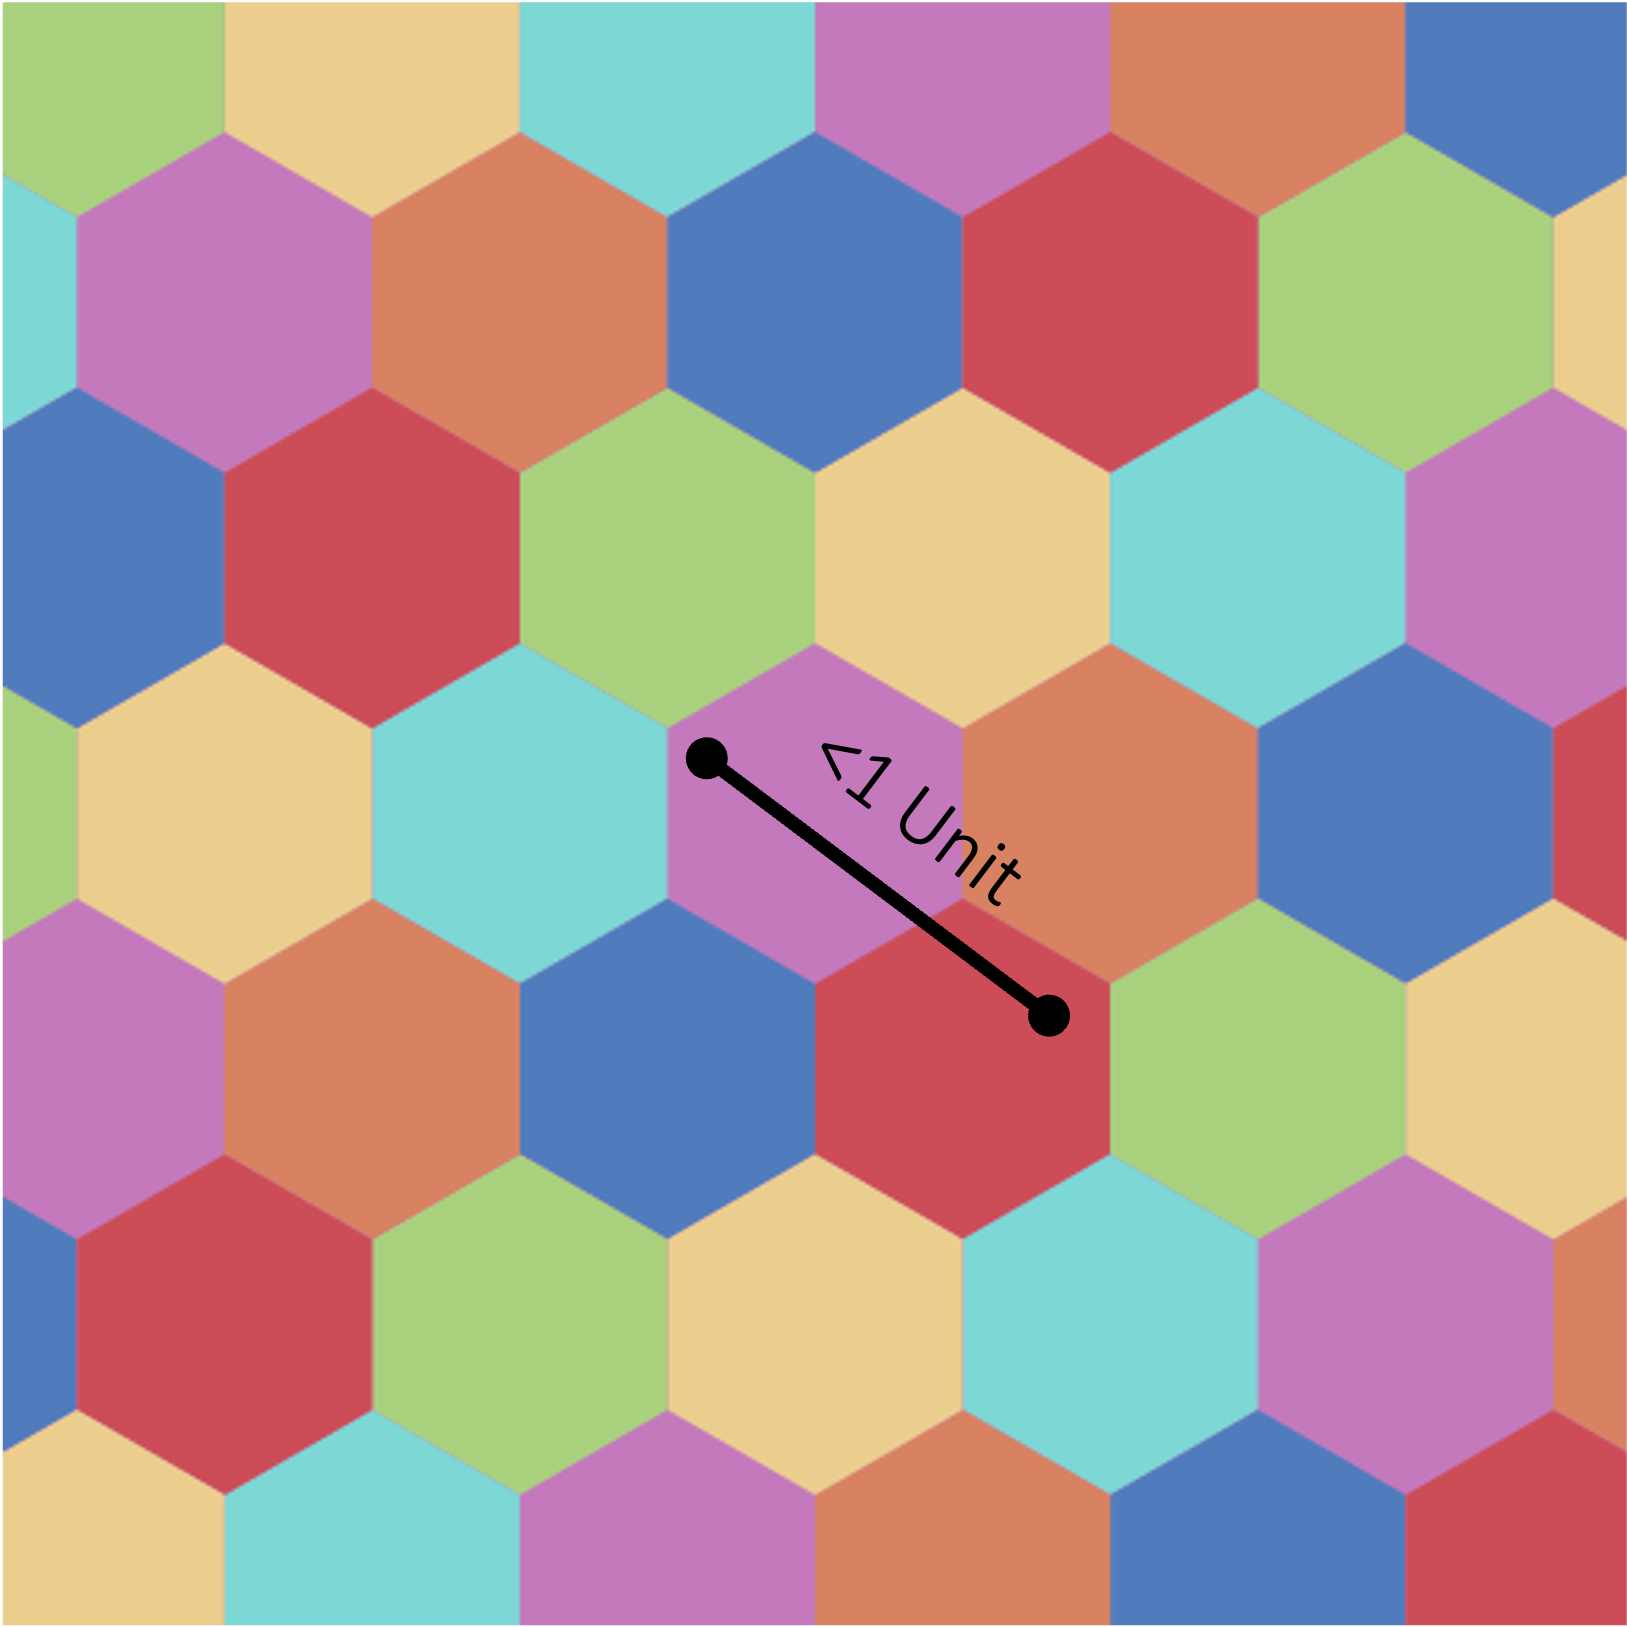
\includegraphics[scale=.5]{HexagonGrid2.png}
			\medspace \medspace \medspace \medspace
			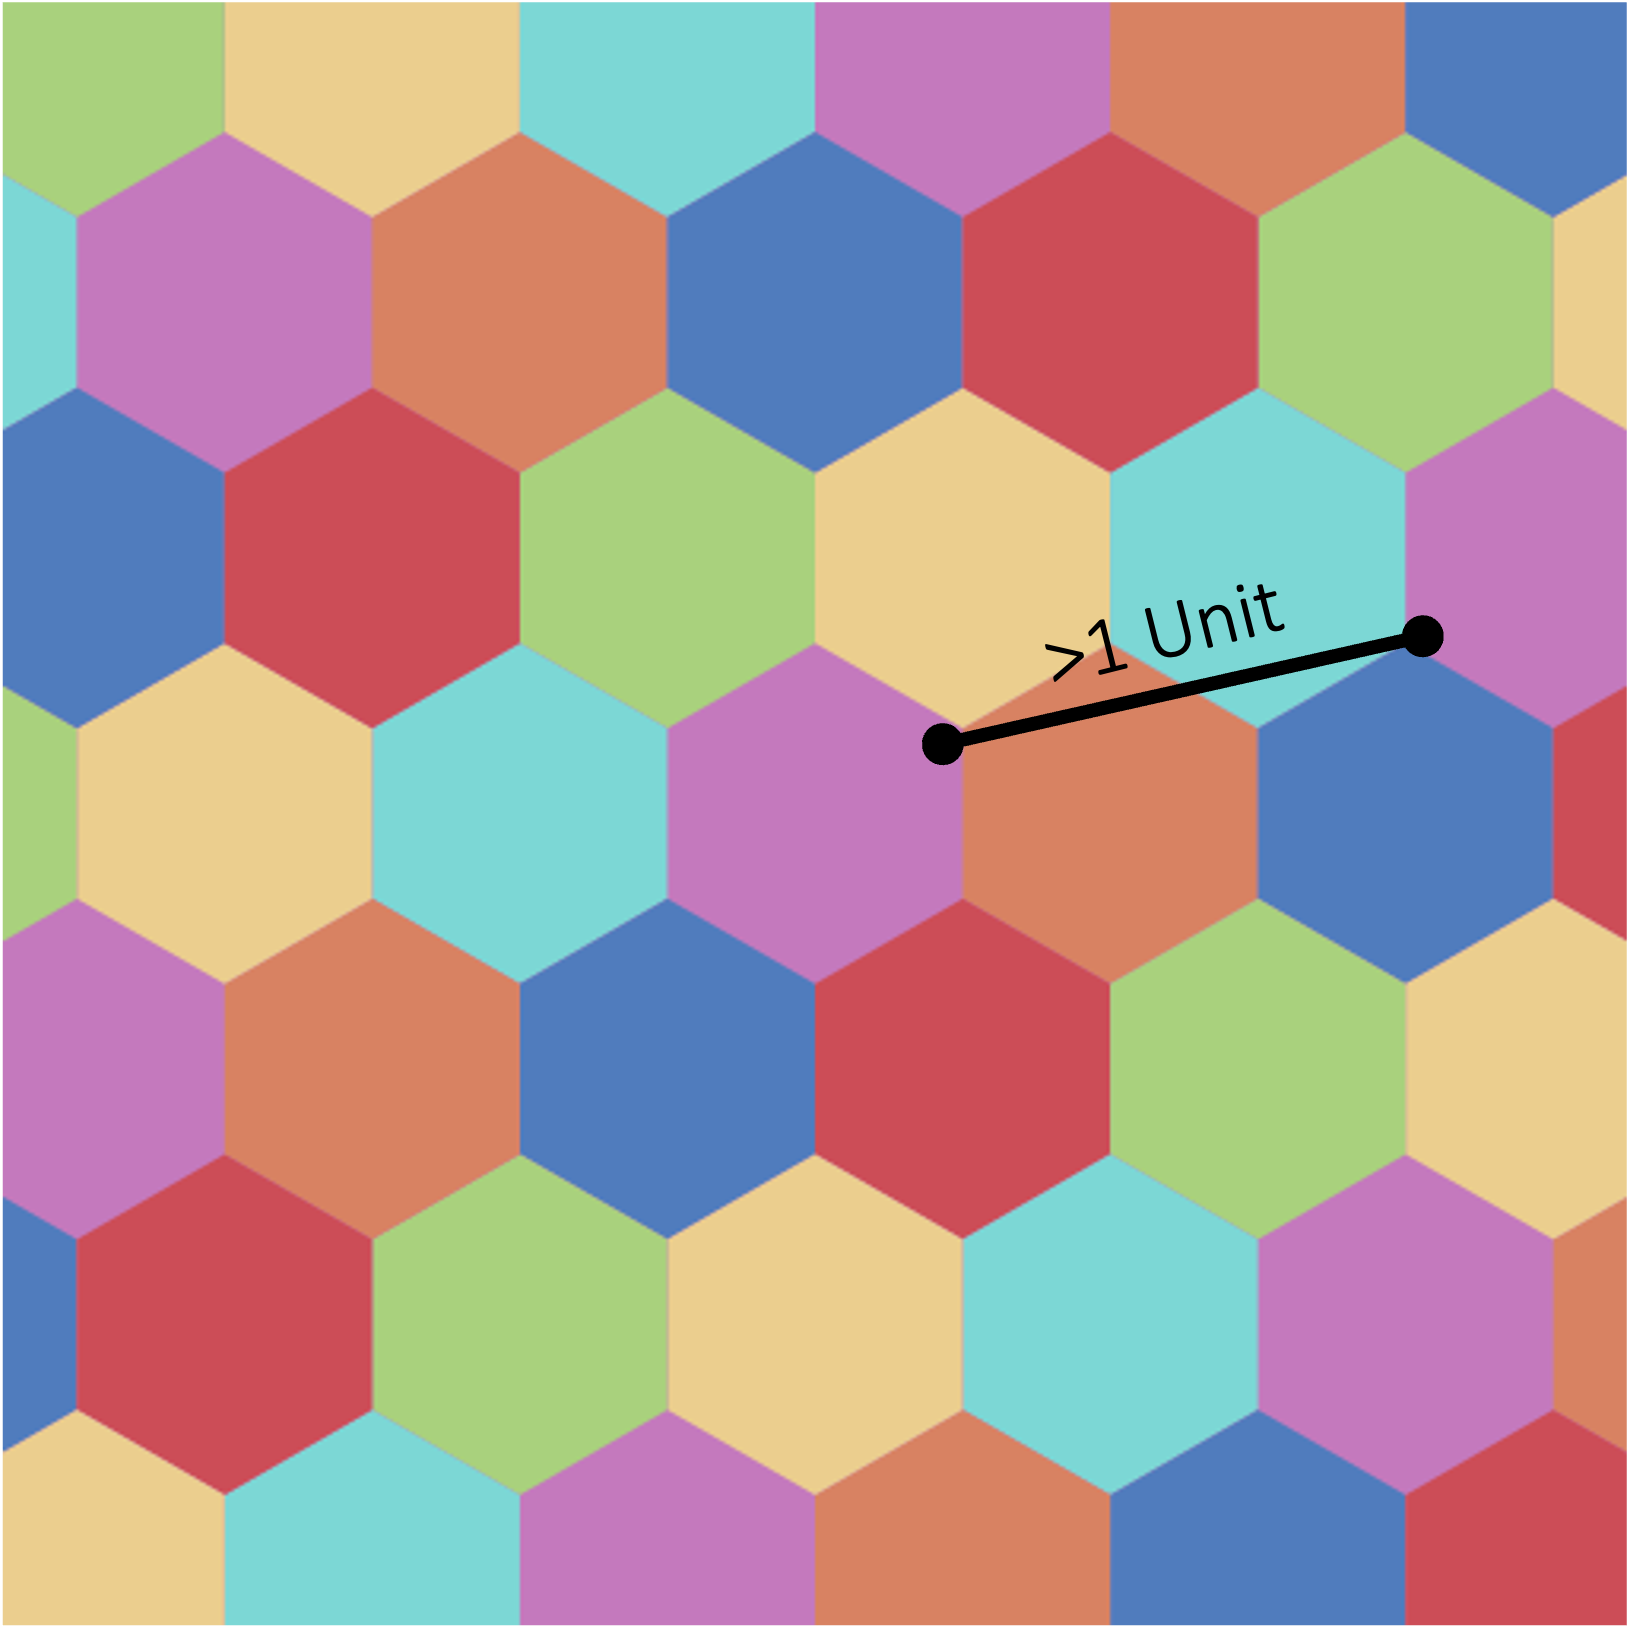
\includegraphics[scale=.5]{HexagonGrid3.png}
			\]
			Moreover, if we make the size of the hexagons such that the length from one vertex of a hexagon to the nearest vertex of a same colored hexagon greater than one unit, every step from a point on the hexagon must never touch a hexagon of the same color.
		\item[(b)]
		To show this has to be done with 3 or more colors we can show this cannot happen with just 2.
		Pretend this is an equalratical triangle representing the walk with each edge of length one:
		% https://q.uiver.app/?q=WzAsMyxbMSwwLCJcXGJ1bGxldCJdLFswLDIsIlxcYnVsbGV0Il0sWzIsMiwiXFxidWxsZXQiXSxbMCwxLCIiLDAseyJzdHlsZSI6eyJoZWFkIjp7Im5hbWUiOiJub25lIn19fV0sWzEsMiwiIiwwLHsic3R5bGUiOnsiaGVhZCI6eyJuYW1lIjoibm9uZSJ9fX1dLFsyLDAsIiIsMCx7InN0eWxlIjp7ImhlYWQiOnsibmFtZSI6Im5vbmUifX19XV0=
\[\begin{tikzcd}
	& \bullet \\
	\\
	\bullet && \bullet
	\arrow[no head, from=1-2, to=3-1]
	\arrow[no head, from=3-1, to=3-3]
	\arrow[no head, from=3-3, to=1-2]
\end{tikzcd}\]
		Then let's color the starting vertex \(r\), and then walk to the top vertex which we color \(b\), then at the third vertex, since we can reach it from either vertex of the  equalratical triangle, must be colored a third color. Therefore, using two colors is not possible, so it must be done with more than 2 colors i.e. 3 or more.
		% https://q.uiver.app/?q=WzAsOSxbMSwwLCJcXGJ1bGxldCJdLFswLDIsInIiXSxbMiwyLCJcXGJ1bGxldCJdLFs0LDIsInIiXSxbNSwwLCJiIl0sWzYsMiwiXFxidWxsZXQiXSxbOCwyLCJyIl0sWzksMCwiYiJdLFsxMCwyLCJcXFJpZ2h0YXJyb3dcXExlZnRhcnJvdyJdLFswLDEsIiIsMCx7InN0eWxlIjp7ImhlYWQiOnsibmFtZSI6Im5vbmUifX19XSxbMSwyLCIiLDAseyJzdHlsZSI6eyJoZWFkIjp7Im5hbWUiOiJub25lIn19fV0sWzIsMCwiIiwwLHsic3R5bGUiOnsiaGVhZCI6eyJuYW1lIjoibm9uZSJ9fX1dLFszLDQsIiIsMCx7InN0eWxlIjp7ImhlYWQiOnsibmFtZSI6Im5vbmUifX19XSxbNCw1LCIiLDAseyJzdHlsZSI6eyJoZWFkIjp7Im5hbWUiOiJub25lIn19fV0sWzUsMywiIiwwLHsic3R5bGUiOnsiaGVhZCI6eyJuYW1lIjoibm9uZSJ9fX1dLFs2LDcsIiIsMCx7InN0eWxlIjp7ImhlYWQiOnsibmFtZSI6Im5vbmUifX19XSxbNyw4LCIiLDAseyJzdHlsZSI6eyJoZWFkIjp7Im5hbWUiOiJub25lIn19fV0sWzgsNiwiIiwwLHsic3R5bGUiOnsiaGVhZCI6eyJuYW1lIjoibm9uZSJ9fX1dXQ==
\[\begin{tikzcd}
	& \bullet &&&& b &&&& b \\
	\\
	r && \bullet && r && \bullet && r && \Rightarrow\Leftarrow
	\arrow[no head, from=1-2, to=3-1]
	\arrow[no head, from=3-1, to=3-3]
	\arrow[no head, from=3-3, to=1-2]
	\arrow[no head, from=3-5, to=1-6]
	\arrow[no head, from=1-6, to=3-7]
	\arrow[no head, from=3-7, to=3-5]
	\arrow[no head, from=3-9, to=1-10]
	\arrow[no head, from=1-10, to=3-11]
	\arrow[no head, from=3-11, to=3-9]
\end{tikzcd}\]
	\end{enumerate}
\end{proof}
	
\end{document}